\documentclass[xcolor=dvipsnames, aspectratio=169]{beamer}

\usetheme{Boadilla}
\usefonttheme{serif}

\usepackage[utf8]{inputenc}
\usepackage[english]{babel}

\usepackage{amsthm}
\usepackage{filecontents}

\usepackage{svg}
\usepackage{color}
\usepackage{graphicx}
\usepackage{tikz}
\usepackage{hyperref}
\usepackage{wallpaper}

\usepackage{verbatim}
\usepackage{subcaption}
\usepackage{svg}
\usepackage{color}


\newcommand{\source}[1]{\begin{textblock*}{4cm}(8.7cm,8.6cm)
    \begin{beamercolorbox}[ht=0.5cm,right]{framesource}
        \usebeamerfont{framesource}\usebeamercolor[fg]{framesource} Source: {#1}
    \end{beamercolorbox}
\end{textblock*}}


% Citation with natbib: 
% Use \citet{} and \citep{} only, not \cite{}
\usepackage{natbib}
\bibliographystyle{abbrvnat}

\usepackage[absolute,overlay]{textpos}
\setbeamercolor{framesource}{fg=gray}
\setbeamerfont{framesource}{size=\tiny}

\DeclareMathOperator*{\argmax}{arg\,max}


\begin{document}
    
    \title[Community Detection for Precipitation Data]{Community Detection for Precipitation Data}
    \author{Johannes Schulz, Adrian Stock}
    \institute[]{Eberhard Karls University Tübingen}
    \date{July 21, 2021}

    \begin{frame}
        \titlepage
    \end{frame}

    \begin{frame}
        \frametitle{Structure}
        
        \begin{large}
            \begin{enumerate}
                \item First look at the data
                \item Network Communities
                \begin{itemize}
                    \begin{large}
                        \item Graph Generation
                        \item Community Detection
                    \end{large}
                \end{itemize}
                \item Results
            \end{enumerate}
        \end{large}
        
    \end{frame}
    
   
    \begin{frame}
        \frametitle{Western Europe}
        \vspace{-.3cm}
        \begin{figure}
            \includegraphics[width=.6\paperwidth]{graphics/considered_region_western_europe.png}
        \end{figure}
    \end{frame}
    
    
    \begin{comment}
            - data source (era5 from copernicus)
            - time and space resolution
            - visualization of data over time/ single point in time
            - some analysis
            
            - add link to data source? I didnt find out how. Maybe add sources slide at the end
    \end{comment}
    \begin{frame}
        \frametitle{Precipitation Data}
        \begin{minipage}[b]{6cm}
            \begin{itemize}
                \item[-] ERA5 dataset from the Copernicus Climate Data Store¹
                \item[-] Spatial resolution: 0.25°x 0.25° 
                \item[-] Temporal resolution: Monthly
                \item[-] 1979 - 2021
            \end{itemize}
        \end{minipage}
        \hspace{.2cm}
        \begin{minipage}{6cm}
            \begin{figure}
            \includegraphics[width=.5\paperwidth]{graphics/cartopy_normalized_data_1979_nov.jpg}
            \end{figure}
        \end{minipage}
        \footnotetext[1]{https://cds.climate.copernicus.eu/cdsapp\#!/dataset/reanalysis-era5-single-levels-monthly-means?tab=overview}
    \end{frame}
    
    
    
    
    \begin{comment}
        \item Intuition for communities
        \item graph generation 
        \item 
    \end{comment}   
    \begin{frame}
        \frametitle{Network Communities}
        \begin{minipage}{.45\paperwidth}
            \begin{itemize}
                \item[-] Communities: Regions with similar characteristics 
                \item[-] In our case: Regions in Western Europe that have similar weather/ precipitation dynamics
            \end{itemize}
        \end{minipage}
        \hspace{.1cm}
        \begin{minipage}{.45\paperwidth}
            \begin{figure}
                \centering
                \includegraphics[width=.4\paperwidth]{graphics/network_communities}
            \end{figure}
        \end{minipage}
        \footnotetext[2]{https://data.graphstream-project.org/talks/CSSS2012/gs-communities.html\#/step-2}
    \end{frame}
    
    \begin{comment}
            -nodes(downsampling)
            -edges(correlation and autocorrelation)
    \end{comment}
    \begin{frame}
        \frametitle{Graph Generation}
        \begin{itemize}
            \item[-] $G=(V,E)$ \pause
            \item[-] Create node for each position in our grid
            \item[] $\Rightarrow |V| = 161 \cdot 221 = 35581$ \pause
            \item[-] $|E| \leq \frac{1}{2} \cdot |V| \cdot (|V|-1) \approx 6.3 \cdot 10^8$ \pause
            \item[-] Connect nodes if statistically significant correlation exists
        \end{itemize}
        
    \end{frame}
    
    
    \begin{frame}{Hypothesis Test}
        %\vspace{-.35cm}
        
        \begin{minipage}{.35\paperwidth}
            \begin{itemize}
                \item[-] $H_0: t_i, t_j \sim \mathcal{N}(0,1)\ i.i.d.$
                \item[-] Significance level $\alpha = 0.001$
            \end{itemize}
            
        \end{minipage}
        \begin{minipage}{.55\paperwidth}
            \begin{figure}[htbp]
            \centering
            \includegraphics[width=.55\paperwidth]{./graphics/hypothesis_testing}
        \end{figure}
        \end{minipage}
        
    \end{frame}
    
    \begin{frame}{Detected Correlations}
        %\vspace{-.2cm}
        \begin{figure}[htbp]
            \centering
            \includegraphics[width=.75\paperwidth]{./graphics/correlations}
        \end{figure}
    \end{frame}
    
    \begin{frame}{Include Correlations in Graph Structure}
    \hspace{.15cm}
    \begin{minipage}{.45\paperwidth}
        \begin{figure}[htbp]
            \includegraphics[width=.45\paperwidth]{graphics/positive_correlations.jpg}
        \end{figure}
    \end{minipage}
    \hspace{.2cm}
    \begin{minipage}{.45\paperwidth}
        \begin{figure}[htbp]
            \includegraphics[width=.45\paperwidth]{graphics/negative_correlations.jpg}
        \end{figure}
    \end{minipage}
    \end{frame}
   
    \begin{frame}{Stochastic Block Modelling}
        \begin{itemize}
            \item[-] Graph $A \in \mathbb{R}^{n\times n}$, parameters $\Theta = \{q \in \mathbb{R}^n, C \in \mathbb{R}^{K\times K} \}$ \pause
            %\item[-] $P((i,j) \in E) = f(q_i, q_j)$
            \item[-]  $\Theta^* = \argmax\limits_\Theta \mathcal{L}(\Theta) = \argmax\limits_\Theta P(A\mid \Theta)$ \pause
            \item[-] Not tractable $\rightarrow$ MCMC approximation of density \pause
            \item[-] Choice of $K$: regularized BIC score 
            \begin{align*}
                \text{BIC} = \log\mathcal{L}(\Theta) + \lambda \cdot |\Theta|
            \end{align*}
        \end{itemize}
    \end{frame}
    
    \begin{comment}
        - communities positive correlations
    \end{comment}
   
    \begin{frame}{Community Detection}
    
        \hspace{.4cm}
        \begin{minipage}{.55\paperwidth}
            \begin{figure}
                \centering
                \includegraphics[width=.55\paperwidth]{graphics/communities_positive_correlations}
            \end{figure}
        \end{minipage}
        \hspace{.3cm}
        \begin{minipage}{.3\paperwidth}
            \begin{figure}
                \centering
                \includegraphics[width=.3\paperwidth]{graphics/adjacency_matrices_with_lines}
            \end{figure}
        \end{minipage}
        
    \end{frame}
    
    \begin{comment}
        - communities negative correlations
    \end{comment}
    \begin{frame}{Community Detection}
    \begin{figure}
        \centering
        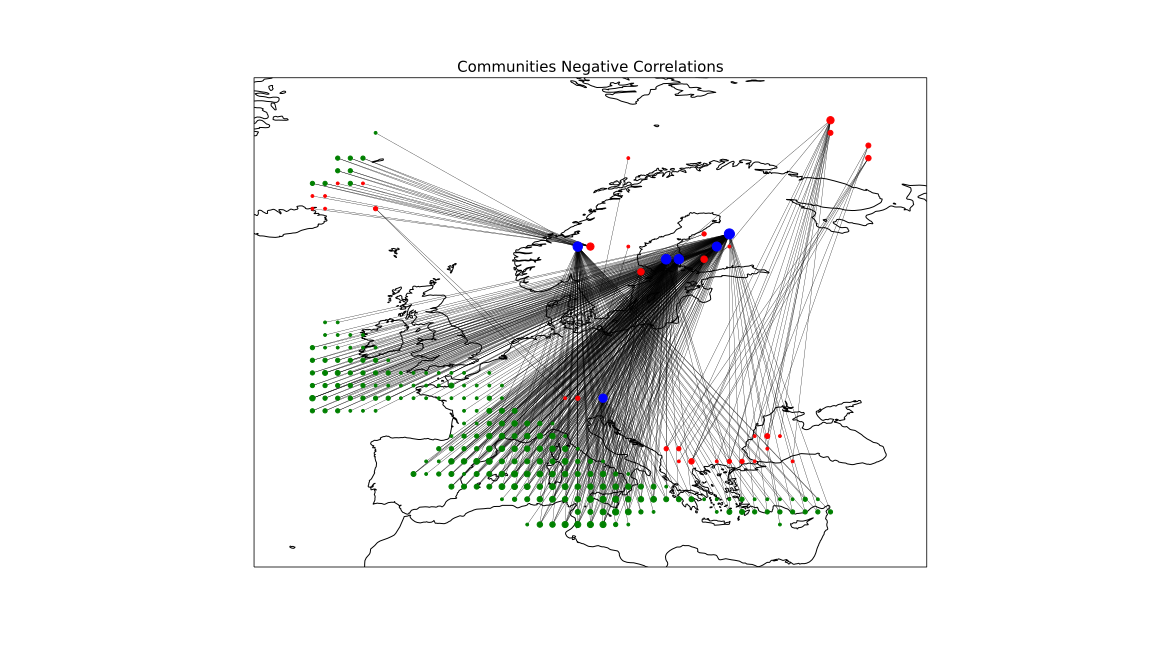
\includegraphics[width=.6\paperwidth]{graphics/communities_negative_correlations.jpg}
    \end{figure}
    \end{frame}
    
    \begin{comment}
        - adjacency matrix
    \end{comment}
 
    
    \begin{comment}
        - We can see NAO "lower part" in the graph with positive correlations
        - We can see that the two parts of NAO anticorrelate
    \end{comment}
    \begin{frame}{Interpretation of Results}
        \hspace{.4cm}
        \begin{minipage}{.55\paperwidth}
            \begin{figure}
                \centering
                \includegraphics[width=.55\paperwidth]{graphics/communities_positive_correlations.jpg}
            \end{figure}
        \end{minipage}
        \hspace{.3cm}
        \begin{minipage}{.3\paperwidth}
            \begin{figure}
                \centering
                \includegraphics[width=.3\paperwidth]{graphics/NAO+.jpg}
            \end{figure}
        \end{minipage}
        
    \end{frame}
    
    \begin{frame}{Interpretation of Results}
        \hspace{.4cm}
        \begin{minipage}{.55\paperwidth}
            \begin{figure}
                \centering
                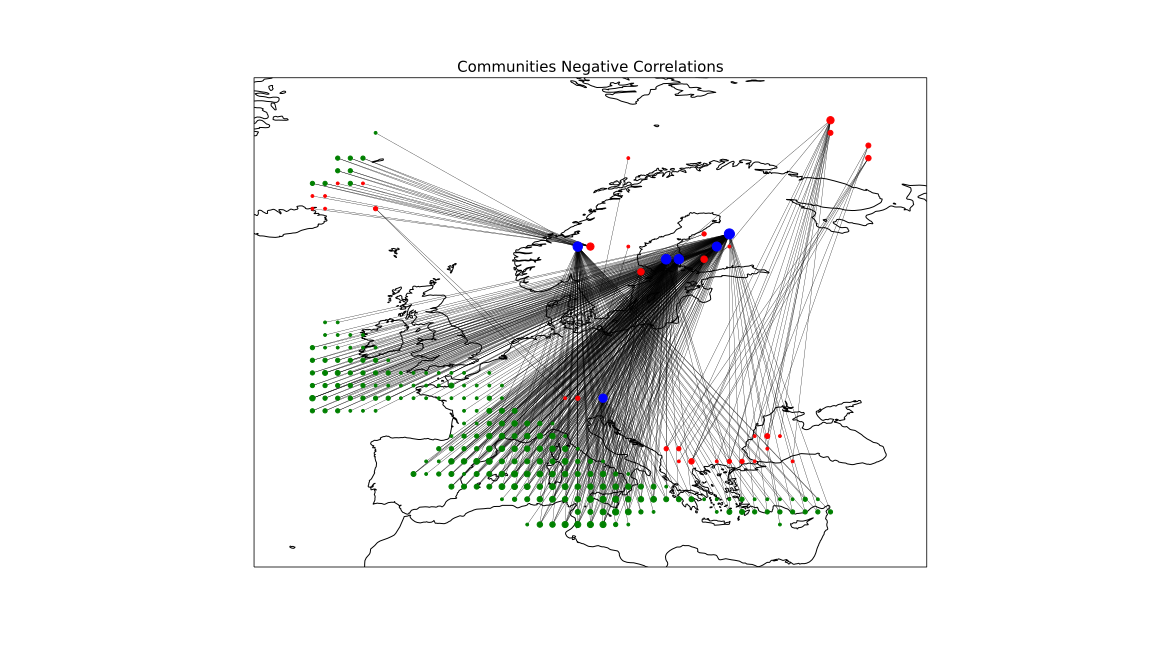
\includegraphics[width=.55\paperwidth]{graphics/communities_negative_correlations.jpg}
            \end{figure}
        \end{minipage}
        \hspace{.3cm}
        \begin{minipage}{.3\paperwidth}
            \begin{figure}
                \centering
                \includegraphics[width=.3\paperwidth]{graphics/NAO+.jpg}
            \end{figure}
        \end{minipage}
        
    \end{frame}
    
    \begin{frame}{}
    \centering
    \begin{Large}
        Thank you very much for your attention!
    \end{Large}
        
    \end{frame}
  
\end{document}
